\section{Software Optimisations \weekDoran{2}}
	\subsection{Profiling}
		\begin{multicols}{2}
			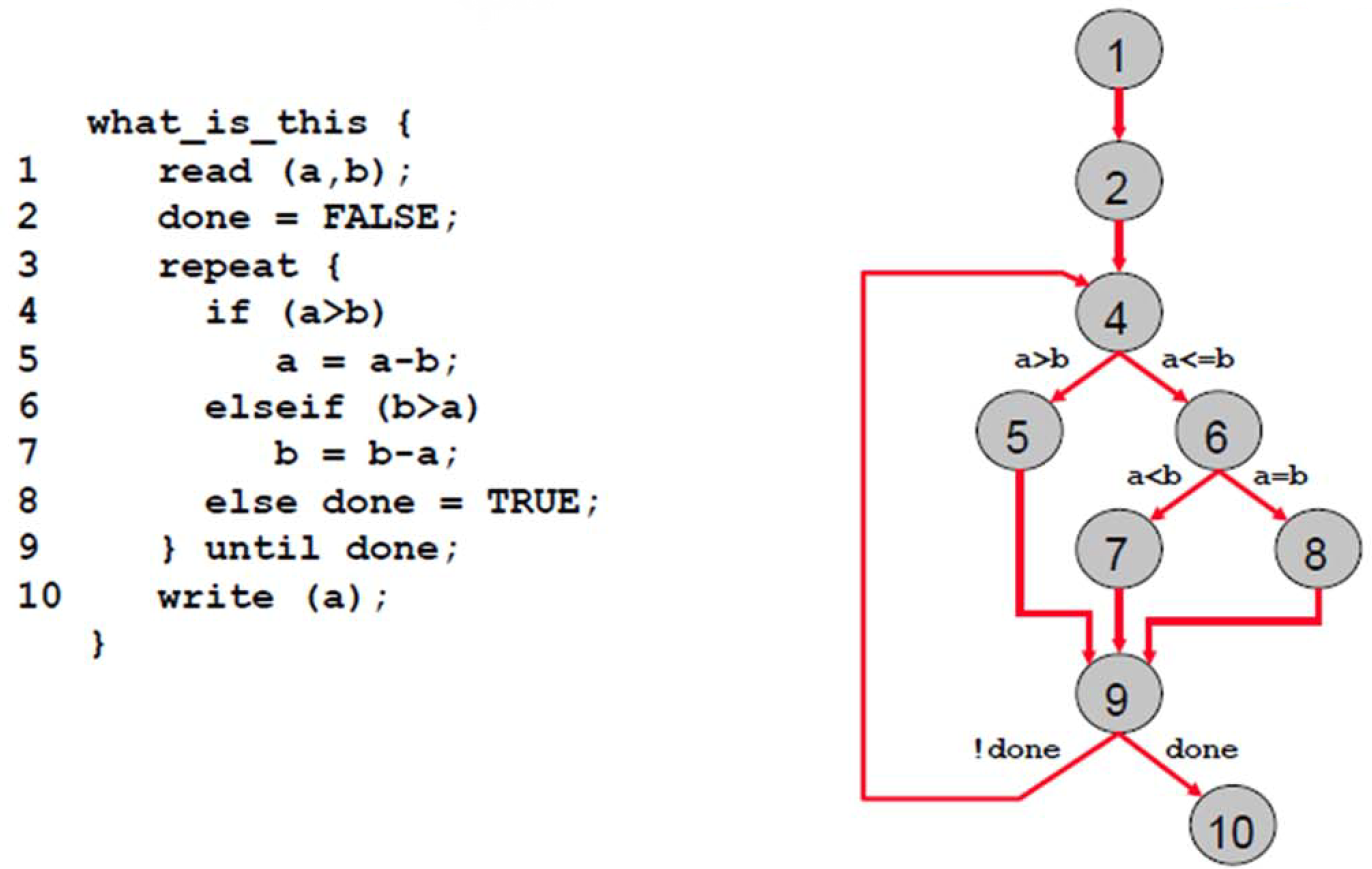
\includegraphics[width=0.4\textwidth]{./pictures/profiling.png} \\
			A code is divided into several blocks. A block is a sequence of instructions, where the control flow enters at the beginning and exits at the end without stopping or branching in between. Then the worst case execution time can be calculated.
			\begin{equation*}
				\begin{aligned}
					WCET &= \sum_{i=1}^{N} c_i * x_i \\
					c_i &= \text{Worst case execution time of block} \\
					x_i &= \text{Number of times the block is executed}
				\end{aligned}
			\end{equation*}			
		\end{multicols}
	
	\subsection{CPU Cycle Time Assumptions For Assembly Instructions}
		{\color{red}\textbf{This is only a rough reference, cycle times depend on many things like architecture, memory proximity and argument types!!}}
		
		\begin{longtable}{|p{0.4\linewidth}|p{0.55\linewidth}|}
				\hline
				\textbf{Instruction}
					& \textbf{Assumed Cycle Time}\\
				\hhline{|=|=|}
				\texttt{MOVE}
					& $1$\\
				\hline
				Load instructions (\texttt{LW, LOAD, LEA})
					& $1$, depending on memory location (or distance)\\
				\hline
				\texttt{CMP}
					& $1$\\
				\hline
				\texttt{ADD}
					& $1$\\
				\hline
				\texttt{SUB}
					& $1$\\
				\hline
				\texttt{MUL}
					& $3$\\
				\hline
				\texttt{DIV}
					& $30..80$\\
				\hline
				\texttt{AND, OR, XOR}
					& $1$\\
				\hline
				Arithmetic shifts (\texttt{ASR/SAR, ASL/SAL})
					& $1$\\
				\hline
				\texttt{CMP}
					& $1$\\
				\hline
				Jumps 
					& $7$ if taken, $1$ if not\\
				\hline
				%\caption{Assumed Cycle Times for Execution Time Calculations}
		\end{longtable}
	
	\subsection{Loop Optimisation \weekPageDoran{2}{20-24}}				
			\begin{longtable}{|>{\bfseries}p{0.3\linewidth}|p{0.65\linewidth}|}
					\hline					
					Loop Fusion / Jamming
						& Combining multiple loops into one.\\
					\hline
					Loop Peeling
						& Take first or last iterations out of loops to simplify.\\
					\hline					
					Loop Unrolling/Unwinding
					& Decrease the number of iterations in a loop by manually executing more than just one of the iterations (i.e. increase step size of the loop to $N$ and do the same operation $N$ times within the loop). Thereby the amount of testing for end of loop condition and pointer arithmetic is decreased. If the loop is completely unrolled, the loop is removed completely and each iteration is inserted one after another.\newline
					\textbf{Loop overhead:}
					\begin{compactitem}
						\item End of loop loop condition check ($\sim 1$ CPU cycle)
						\item Jumps ($\sim 7$ CPU cycles if taken, $1$ if not)
						\item Increment loop index ($\sim 1$ CPU cycle)
					\end{compactitem} \\[-\normalbaselineskip]
					\hline
					Loop Hoisting
					& Take invariant condition out of loop (i.e. something that doesn't change once you're in the loop).\\
					\hline
			\end{longtable}
		
		\begin{multicols}{3}		
			\lstinputlisting[style=C]{./src/sobelOriginal.c} \ \\
			\lstinputlisting[style=C]{./src/sobelUnrolled.c} \ \\ \ \\
			\lstinputlisting[style=C]{./src/sobelPeeling.c}
		\end{multicols}	
		
	\subsection{In-lining}
		Replacing the function call with the body of the function. Excess inlining can cause speed issues due to code taking too much space in the memory (or cache).